% This is my template for presentations of diploma
% All slides in code separated by line

\documentclass[compress]{beamer}    % [ucs] makes Cyrillic fonts visible in index 
\usepackage{beamerthemeshadow}          % use <beamerthemeshadow> theme
% \usepackage{default} 			% use empty/default style, usefull for printing 
\usepackage[T2A]{fontenc}
\usepackage[utf8]{inputenc}             % set encoding
\usepackage[english]{babel}
\usepackage{amssymb,amsfonts,amsmath}
\usepackage{cite,enumerate,float,indentfirst}
\usepackage{graphicx,epstopdf}          % epstopdf-convert eps files to pdf
\usepackage{textcomp}

\graphicspath{{figs/}}       % look up folders for figures
\setbeamertemplate{footline}[page number] % insert number of slides
\usepackage{color}                      % you can colour your formulas with this, just use ${\color{red} E=mc^2}$
\usepackage{helvet} 	                % set font family for whole document
\usefonttheme[onlymath]{serif}          % Set font family only for math mode



\beamertemplatenavigationsymbolsempty   % hide naviagation bar

% Setup caption near figures, prticulary make font smaller
\usepackage[ font=small]{caption}
\captionsetup{font=scriptsize,labelfont=scriptsize}



% If you want divide slide on two parts just use code:
% \begin{columns}[t]
% \begin{column}{5cm}
%  some data in column 1
% \end{column}
% \begin{column}{5cm}
%  some data in column 2
% \end{column}
% \end{columns}

% If you want to make theorem or emphasize some info, use next code:
% \begin{block}{title of block}
% Some data in block, feel free to add formulas,tables or figures here.
% \end{block} 

% use \begin{frame}[shrink=5] in case if you need insert more text in slide

\begin{document}
\title{Combined Complementary Filter For Inertial Navigation System}  
% \author{доповідач:Микола Новік\\ керівник: Мар’ясова Т.І.}
\author{M.K. Filiashkin \\ M.V.Novik}
\date{\today} 
%%%%<<<<<<<<<<<<<<<<<<<<<<<<<<<<<<<<<<<<<<<<<<<<<<<<<<<<<<<<<<<<<<<<<<<<<<<<<<<<<<<
% First Slide, title page
\begin{frame}
\titlepage
\end{frame}

%%%%<<<<<<<<<<<<<<<<<<<<<<<<<<<<<<<<<<<<<<<<<<<<<<<<<<<<<<<<<<<<<<<<<<<<<<<<<<<<<<<
% Intro
\section{Introduction} 
\subsection{Introduction} 
\begin{frame}\frametitle{Introduction}
\small
\beamerbutton{\smallПостановка задачі}: дослідження можливостей комплексування навігаційної інформації двох систем, що є на борту сучасного літака: безплатформенної інерціальної навігаційної системи і супутникової високоточної навігаційної системи.\\
\centering \line(1,0){200}

\begin{block}<+->{В результатi комплексування IНС та СНС досягаються:}
\tiny
\begin{enumerate}
\item  пiдвищення точностi визначення координат, висоти, швидкостi i часу споживача;
\item  уточнення кутiв орiєнтацiї (курсу, крену i тангажа);
\item  оцiнка й уточнення параметрiв калiбрування навiгацiйних датчикiв,
таких, як дрейфи гiроскопiв, масштабнi коефiцiєнти, зсуви нуля акселерометрів тощо;
\item  забезпечення на цiй основi безперервностi навiгацiйних визначень на всiх етапах руху, у тому числi i при тимчасовiй непрацездатностi приймача СНС у випадках впливу завад або енергiйних маневрiв ЛА.

\end{enumerate}
\end{block}

\end{frame} 
%%%%<<<<<<<<<<<<<<<<<<<<<<<<<<<<<<<<<<<<<<<<<<<<<<<<<<<<<<<<<<<<<<<<<<<<<<<<<<<<<<<
\section{Complementary filter} 
\begin{frame}%[plain]
\frametitle{Complementary filter}
\small
\begin{figure}[!t]
\centering
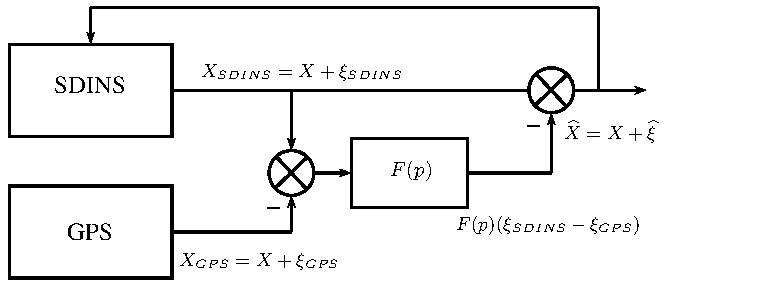
\includegraphics[scale=0.5]{f1}
\captionsetup{font=scriptsize,labelfont=scriptsize}
\caption{\tiny Complementary filter}
\label{fig:compl}
\end{figure}
% \begin{columns}[t]
% \begin{column}
\begin{equation}
\displaystyle F(p) = \left\{ 
    \begin{array}{ll}
       \displaystyle \frac{1}{T_{1} p+1} & \mbox{if $t_{up} \le T_{1}$};\\
       \displaystyle \frac{T_{2} p+1}{(T_{2} p+1)(T_{2} p+1)(T_{2} p+1)} & \mbox{if $T_{1} <t_{up} \le T_{2}$};\\
       \displaystyle \frac{T_{3} p+1}{(T_{3} p+1)(T_{3} p+1)(T_{3} p+1)}& \mbox{if $T_{2} < t_{up}$}.
    \end{array} 
\right.
\label{eq:comp_f}
\end{equation}
% \end{column}
% \end{columns}
\end{frame}


%%%%<<<<<<<<<<<<<<<<<<<<<<<<<<<<<<<<<<<<<<<<<<<<<<<<<<<<<<<<<<<<<<<<<<<<<<<<<<<<<<<
\begin{frame}
\frametitle{Simple INS}
\begin{block}{Equation of Motion}
\begin{equation}
\begin{array}{l}
  \displaystyle \dot{\varphi }=\frac{V_{N} }{R_{E} +h} ; \dot{h}=V_{U} ; \dot{\vartheta }=\omega -\frac{V_{N} }{R_{E} +h} ;\\
  \displaystyle \dot{V}_{N} =a_{N} -\frac{V_{N} }{R_{E} +h} V; \dot{V}_{U} =a_{U} +\frac{V_{N} }{R_{E} +h} V_{N} -g;\\
  \displaystyle a_{N} =a_{y} \cos \vartheta -a_{z} \sin \vartheta ; a_{U} =a_{y} \sin \vartheta +a_{z} \cos \vartheta ;\\
  \end{array} 
  \label{eq:ins}
\end{equation}
\end{block}
$\varphi$,$h$- latitude and height; \\
$V_{N}$, $V_{U}$- North and Up velocity; \\
$a_{N}$, $a_{U}$ - North and Up acceleration; \\
$a_{y}$, $a_{z}$ - acceleration in body frame (accelerometers output); \\
$\vartheta$ - pitch angle;$\omega $- angular velocity in body frame (gyro output); \\
$R_{E}$- Earth radius;
\end{frame}

%%%%<<<<<<<<<<<<<<<<<<<<<<<<<<<<<<<<<<<<<<<<<<<<<<<<<<<<<<<<<<<<<<<<<<<<<<<<<<<<<<<
\subsection{Sensors Parameters}
\begin{frame}
\frametitle{Sensors Parameters}
\begin{block}{Sensors}
\begin{table}%[H]
\centering
\centering
\renewcommand{\arraystretch}{1.3}
  \caption{Simulation Parameters}
    \begin{tabular}{|l|p{50mm}|} \hline 
      Parameter & Value \\ \hline  \hline 
      Gyro bias & $100^{\circ } /hr$ \\ \hline 
      Angular random walk & $1.2^{\circ } /\sqrt{hr} $ \\ \hline 
      Accelerometer bias & $10^{-2} g$ \\ \hline 
      Velocity random walk & $0.18m/s/\sqrt{hr} $ \\ \hline 
      GNSS position precision & $7m(1\sigma )$ \\ \hline 
      GNSS velocity precision & $0.05m/s(1\sigma )$ \\ \hline 
    \end{tabular}
  \label{tab:sim}
\end{table}
\end{block}
\end{frame}
%%%%<<<<<<<<<<<<<<<<<<<<<<<<<<<<<<<<<<<<<<<<<<<<<<<<<<<<<<<<<<<<<<<<<<<<<<<<<<<<<<<
\subsection{Estimation error of positon and velocity}
\begin{frame}
\frametitle{Estimation error of positon and velocity}
\noindent

\begin{figure}[l]
  \centering
  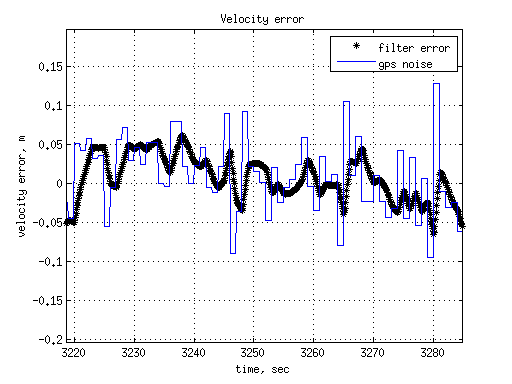
\includegraphics[scale=0.41]{vn_err_of_err}
  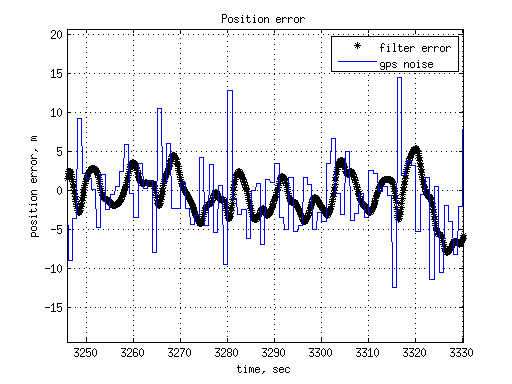
\includegraphics[scale=0.41]{phi_err_of_err}
  \caption{Estimation error of positon and velocity}
  \label{fig:comp_pos}
\end{figure}
\end{frame}
%%%%<<<<<<<<<<<<<<<<<<<<<<<<<<<<<<<<<<<<<<<<<<<<<<<<<<<<<<<<<<<<<<<<<<<<<<<<<<<<<<<
\subsection{INS error of positon and velocity}
\begin{frame}
\frametitle{INS error of positon and velocity}
\noindent

\begin{figure}[l]
  \centering
  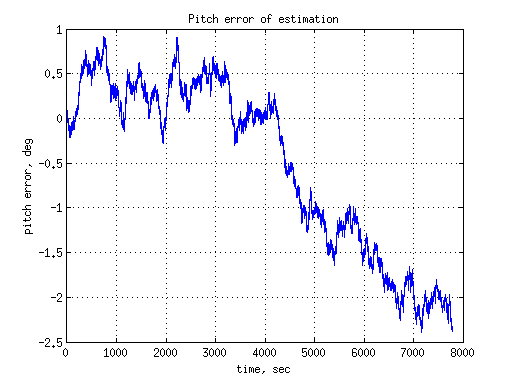
\includegraphics[scale=0.41]{theta_err_of_err}
  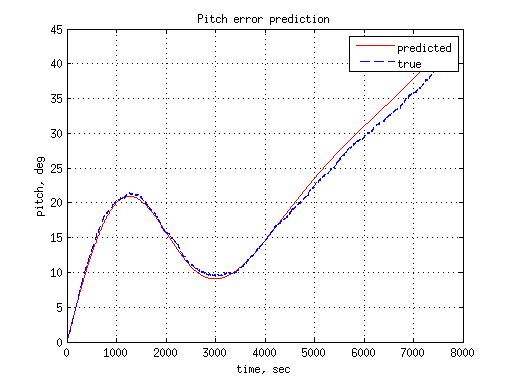
\includegraphics[scale=0.41]{theta_err}
  \caption{INS error of positon and velocity}
  \label{fig:comp_pos}
\end{figure}
\end{frame}
%%%%<<<<<<<<<<<<<<<<<<<<<<<<<<<<<<<<<<<<<<<<<<<<<<<<<<<<<<<<<<<<<<<<<<<<<<<<<<<<<<<
\subsection{INS attitude error in case of 10\% error in initial condition}
\begin{frame}
\frametitle{INS attitude error in case of 10\% error in initial condition}
\noindent

\begin{figure}[l]
  \centering
  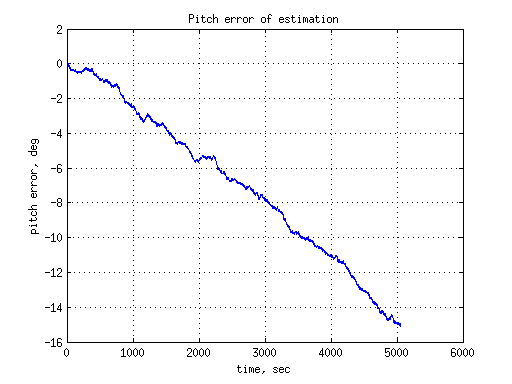
\includegraphics[scale=0.41]{theta_err_of_err_2}
  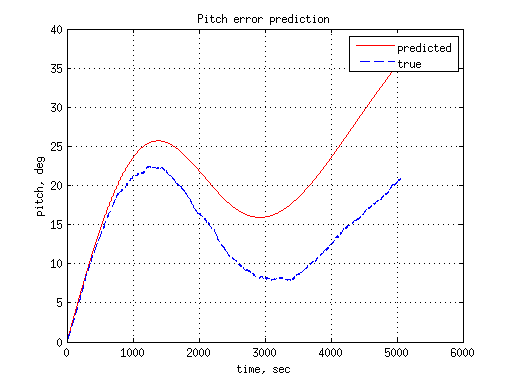
\includegraphics[scale=0.41]{theta_err_2}
  \caption{Prediction of  INS attitude error in case of 10\% error in initial condition for gyro bias}
  \label{fig:comp_pos}
\end{figure}
\end{frame}
%%%<<<<<<<<<<<<<<<<<<<<<<<<<<<<<<<<<<<<<<<<<<<<<<<<<<<<<<<<<<<<<<<<<<<<<<<<<<<<<<<
% Last slide... with Easter Egg
\section{The End} 
\begin{frame}%[plain]
\begin{block}{sudo rm -rf / }
  \centering
  Chears! \\
  @isinf\\
  https://github.com/phen0m

\end{block}
\end{frame}

%%%%<<<<<<<<<<<<<<<<<<<<<<<<<<<<<<<<<<<<<<<<<<<<<<<<<<<<<<<<<<<<<<<<<<<<<<<<<<<<<<<
\end{document}